\chapter{Introduction} % Main chapter title
\label{ch:intro} % Change X to a consecutive number; for referencing this chapter elsewhere, use \ref{ChapterX}

Augmented Reality (AR) is technology that enables the seamless overlay of virtual images on the real world so that both real and virtual can be seen and interacted with at the same time. \cite{azuma1997survey} defined AR as the coexistence of the virtual world and the real world "it would appear to the user that the virtual and real objects coexisted in the same space" (Figure \ref{fig:video-see-through}). Milgram \cite{Milgram1995a} defined the mixed reality (MR) continuum and placed augmented reality (mostly real content overlaid by virtual content) between virtual reality (VR) where full immersion of virtual contents and augmented virtuality (AV) where mostly virtual content overlaid by real content (Figure \ref{fig:mr-continuum}). 

\begin{figure}
    \centering
    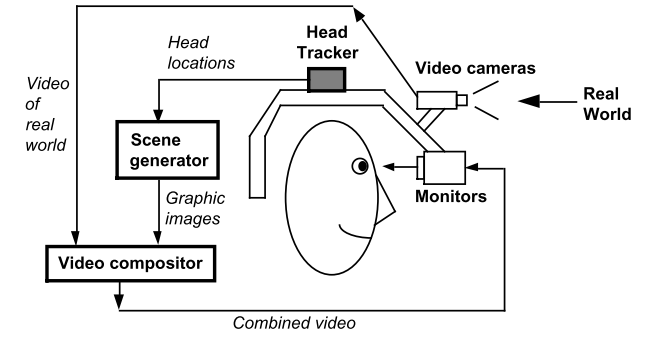
\includegraphics[width=.8\linewidth]{images/video-see-through-ar.png}
    \caption{video see-through AR display}
    \label{fig:video-see-through}
\end{figure}

\begin{figure}
    \centering
    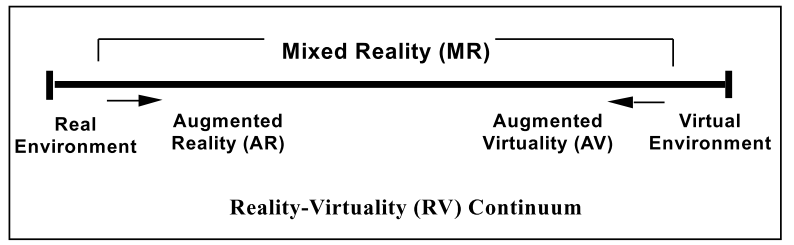
\includegraphics[width=.8\linewidth]{images/mixed-reality-continuum.png}
    \caption{Mixed reality continuum}
    \label{fig:mr-continuum}
\end{figure}

\cite{Zhou2008, Kim2018} looked at trend of augmented reality in the academic conference ISMAR and looked at trends in the research community and reported "a dramatic increase of commercial interest in AR/MR" and "AR technology will continue to develop even more dynamically and effectively over the next ten years, toward the vision of pervasive presence in our daily lives.". AR displays are getting more affordable with better rendering and registration techniques. Also, AR displays are getting untethered enabling mobile AR applications, and self-contained displays are entering the market.

\section{Problem Statement}

This PhD thesis addresses the problems of: 
(1) using visualising and interacting with social contacts through wearable augmented reality displays. 
(2) displaying a large amount of 3D content of sharing social data that is overlaid over a limited available physical space through wearable AR devices. 
(3) defining and exploring the best ways to use wearable AR devices to connect with social networks.
The focus of this thesis is on enabling the use of wearable AR for sharing social experiences. 

% - The potential for AR to be a social sharing platform. \\
% - Sharing social experiences was not fully addressed in the research community

With major industry players (e.g. Microsoft, Facebook and Magic Leap) supporting Augmented Reality (AR), there is a potential use of AR/VR could be for connecting with social networks. Just as people today use their mobile phones to connect with hundreds or thousands of "friends", wearable AR displays could be used to connect with friends and view and interact with their shared information.

Applications for Social VR and 360 videos have been introduced on new VR headsets. For instance, Facebook Spaces\footnote{https://www.facebook.com/spaces} allows VR users to connect with friends and family and share 360 photos and take selfies. AltSpaceVR\footnote{https://altvr.com/} was acquired by Microsoft and enable more diverse hand-held and wearable devices to be used for social connection with others. Most recently Magic Leap's Avatar Chat\footnote{https://www.magicleap.com/stories/blog/connect-with-friends-with-avatar-chat} offers similar experiences where avatars representing social friends are displayed in an AR space (Figure \ref{fig:ml-avatar-chat}). 


\begin{figure}
    \centering
    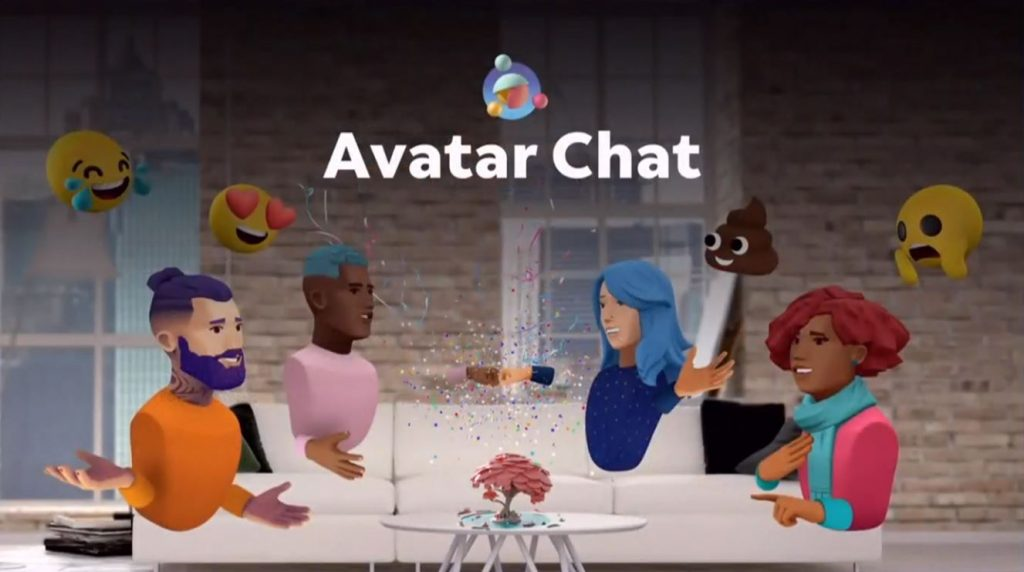
\includegraphics[width=.8\linewidth]{images/magic-leap-avatar-chat.jpg}
    \caption{Magic Leap - Avatar Chat}
    \label{fig:ml-avatar-chat}
\end{figure}


Previously, handheld AR systems have been used to view social networks in a number of different ways. For example, Presslite's Twitter 360\footnote{https://www.youtube.com/watch?v=5w7EAz8-uwU} shows virtual tweets overlaid on the real world at the locations of the people that sent them (see figure \ref{fig:presslite}), and early versions of Junaio\footnote{https://en.wikipedia.org/wiki/Junaio} allowed people to drop virtual messages and pictures in the real world, as did the popular application Sekai Camera\footnote{https://www.youtube.com/watch?v=oxnKOQkWwF8}. Most of these applications were focused on asynchronous collaboration, enabling people to post virtual messages in space which can later be browsed and retrieved by other users. 

\begin{figure}
    \centering
    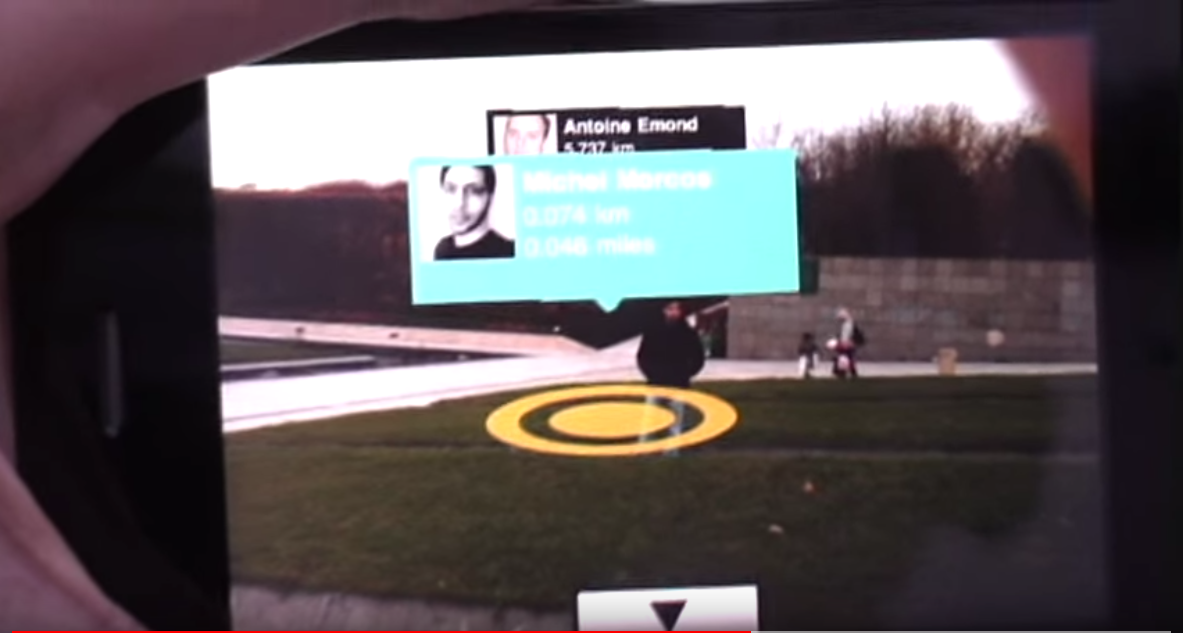
\includegraphics[width=.8\linewidth]{images/Presslite-twitter-360.PNG}
    \caption{Presslite's Twitter 360 AR interface}
    \label{fig:presslite}
\end{figure}

However similar technology could also be used for live synchronous collaboration such as live video avatar sharing  \cite{Billinghurst2002}, or sharing realistic 3D models superimposed over the real world \cite{Fanello2016}, or by using virtual avatars to show a live view of remote collaborators and their surrounding space as in the Holoportation system \cite{Fanello2016} (see figure \ref{fig:holoportation}).

\cite{Peddie2017} reviewed the historic uses of wearable displays and AR displays. 

\begin{figure}
    \centering
    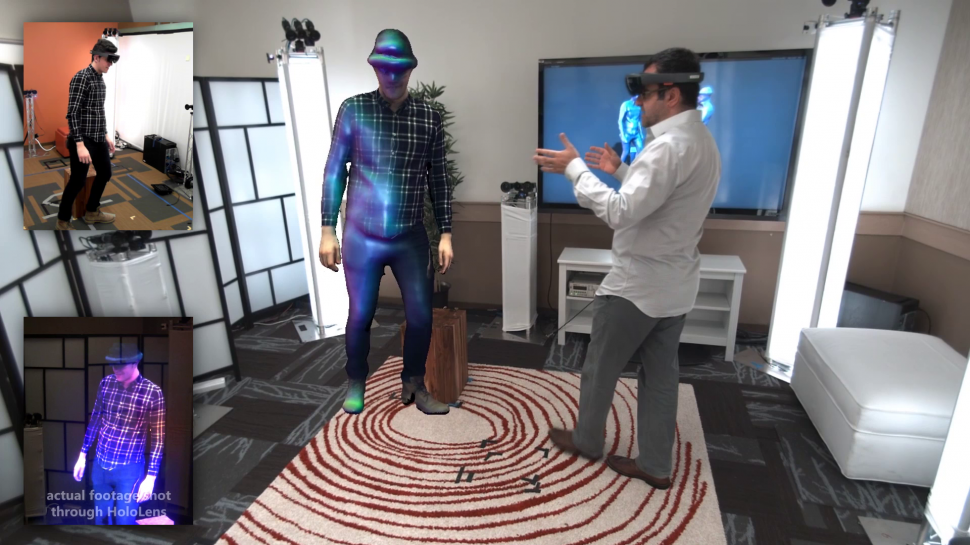
\includegraphics[width=.8\linewidth]{images/holoportation.png}
    \caption{Holoportation}
    \label{fig:holoportation}
\end{figure}

By using a wearable AR display like the Microsoft HoloLens\footnote{https://www.microsoft.com/en-nz/hololens}, it could be possible for the user to see an AR representation of their social network visible at all times. However, this raises the question of how to visually represent the user's contacts in the network. For example, if a user has a large social network with hundreds of contacts available, visually representing each of them might clutter the user's visual space.

\section{Research Questions}

This thesis targets the future where AR devices are used every day, and social networks are visualised in the AR view. The overarching research question is how to share social experiences on AR devices. So we address the following research questions: 

\begin{itemize}
    % (chapter 3 - Social AR continuum)
    \item RQ1: How to represent social networks and shared social data on wearable AR devices 
    
    \item RQ1(option 2): What dimensions/factors/parameters in sharing social experiences on wearable AR devices 
    
    % (chapter 4 - annotation continuum)
    \item RQ2: How to represent annotations/tags on shared social experience through wearable AR devices
    
    % (chapter 5 - Sharing data continuum)
    \item RQ3: How to share virtual objects/data with our social network through wearable AR 
    
    % (chapter 6 - visualising social contacts) 
    \item RQ4: How to visualise our social contacts as virtual avatars through wearable AR devices

\end{itemize}

To answer the research questions, this thesis explores how wearable AR can be used for sharing social experiences. These explorations identify the parameters at which AR sharing for social reasons happen. Once the parameters are defined, we build a few system prototypes as a proof of concept of the experience or the interaction design. We then run user studies to test the objectives of the system with human participants. We observe their behaviour and report on the results of these experiments. 

\section{Contributions}

The followings summarise the contributions of this thesis as the following: 

\begin{enumerate}
    \item Identifying parameters and dimensions of the social AR continuum. This thesis' main contribution is defining the social AR continuum space which consists of a set of parameters that define the space of sharing social experiences through AR wearable/hand-held devices. We define the space of AR continuum by exploring the main parameters that can be varied based on social proximity. These parameters are grouped into the following categories 1) self and other, 2) shared objects and annotation and 3) surrounding environments. Under each of these categories, we define the dimensions of variables that affect the shared social experience.
    
    \item The implementation of the AR experience user interface. For each dimension defined on the continuum, we built a software and hardware prototype to test the user interface design with human subjects. The implementation details are described in the thesis for future studies purposes.
    
    \item User studies and evaluation to validate the parameters of the social AR continuum.  we built a prototype and run a user-study/focus-group to validate the dimensions on the social AR continuum. 
    
    \item High-level design guidelines for interface designers who are building social sharing experiences on AR devices. One of the outcomes of defining the social AR continuum and validating these dimensions is that it can serve as a high-level experience design guidelines that help individual/organisations to create AR experiences for social sharing and connection purposes.
\end{enumerate}

In summary, this thesis helps to increase the understanding of how to share social experiences through AR devices. The results of the user experiments conducted throughout this research help identifying the impact of the social AR continuum parameters on presence, user engagement and user interface usability, which serves as a guideline for future designs. 

The rest of the thesis is organised as follows: Chapter \ref{ch:continuum} describes the social AR continuum and the parameters/ dimensions involved. Chapter \ref{ch:annotation} describes the shared data and annotation continuum including different implementation of shared annotation and awareness cues on different platforms (handheld and wearable). Chapter \ref{ch:data} describes the surrounding environment continuum including shared 360 videos and 30 captured spaces. Chapter \ref{ch:contacts} describes the continuum of self and others of representing social contacts networks on AR devices. The following diagram (Figure \ref{fig:thesis-outline}) shows the structure of the thesis and how it answers the research questions. 

\begin{figure}
    \centering
    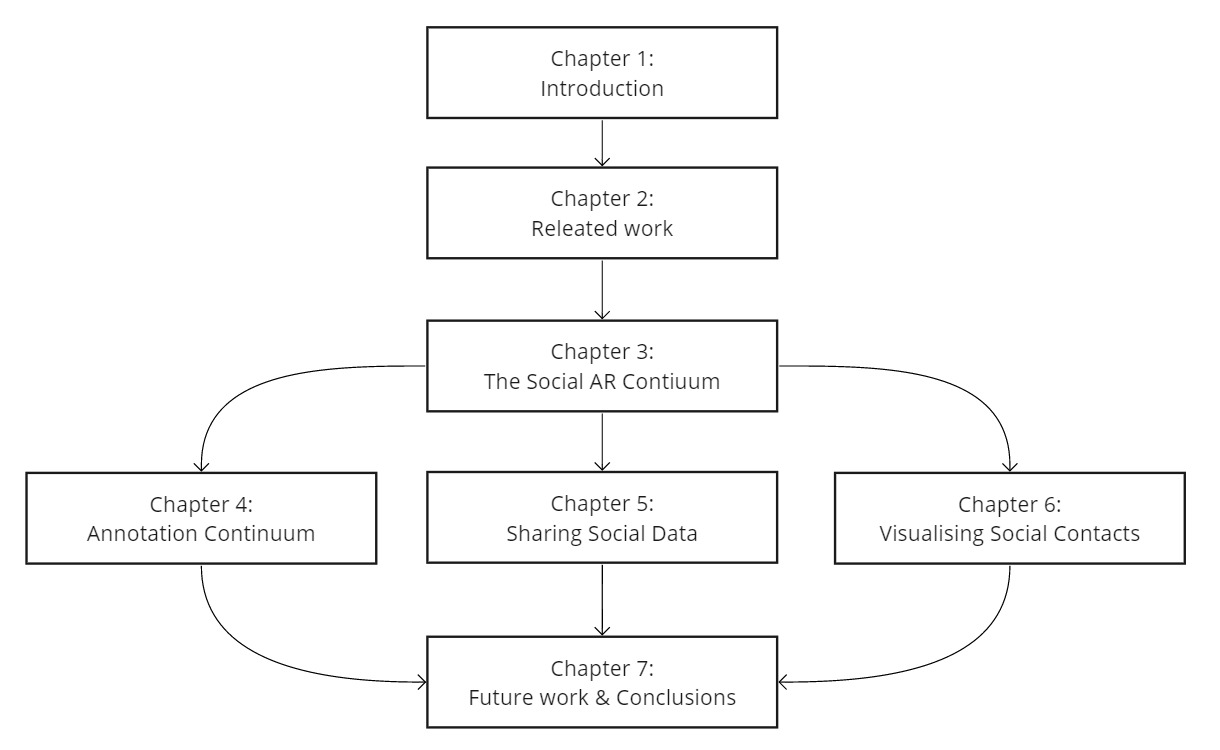
\includegraphics[width=.8\linewidth]{images/thesis-outline.png}
    \caption{Thesis outline}
    \label{fig:thesis-outline}
\end{figure}

\section{Selected Publications}

Most of the work of this thesis has been submitted, peer-reviewed and published at scientific conferences specialising in AR, HCI and Computer Graphics fields. This list contains selected publications that are relevant to this thesis. 

The following publication defines the concept of the social AR continuum and describes a focus group and a user study implementing visualising social contacts through AR headset, and answering RQ1. 

\begin{itemize}
    \item{ \fullcite{Nassani2017a}}
\end{itemize}

The following publications focus on placing AR annotations/tag on shared 360 panorama and video streaming contents, and answering RQ2.

\begin{itemize}
    \item{ \fullcite{Nassani2016}}
    \item{ \fullcite{Nassani2015}}
    \item{ \fullcite{Nassani2015a}}    
    \item{ \fullcite{Reichherzer2014}}
    \item{ \fullcite{Billinghurst2014}}
\end{itemize}

The following publications focus on shared surrounding environments and changing the level of details based on social proximity, and answering RQ3.

\begin{itemize}
    \item{ \fullcite{Nassani2018a}}
    \item{ \fullcite{Nassani2018b}}
    % \item{ \fullcite{Nassani2018c}} -- frontier paper rejected
\end{itemize}

The following publications focus on visualising social contacts based on social proximity, and answering RQ4. 

\begin{itemize}
    \item{ \fullcite{Nassani2017b}}
    \item{ \fullcite{Nassani2017}}
\end{itemize}

The above publications help to answer the research questions of thesis including how to share social experiences on AR devices for each category on the social AR continuum. 


% \todo[inline]{Mark: In the remainder of the thesis we first review related work and explain the research gap that our work files (section 2). Then [put  more here – summarise the thesis structure] }

% \todo[inline]{[You may also want to put together a  thesis outline chart. Basically showing the experiments you conducted and  prototypes you developed and  how these  contribute to addressing  the research questions that you’ve raised. This is helpful if you have a lot of material to report on, so the reviewers can understand how it all fits together] }